\documentclass[tikz,border=8pt]{standalone}
% Shared look for every TikZ diagram. Load with \input{../../tools/tikz-style.tex}
\usepackage[T1]{fontenc}
\usepackage{lmodern}
\renewcommand{\sfdefault}{lmr}  % diagrams use the same serif as the text
\usetikzlibrary{arrows.meta, positioning, shapes.geometric, calc, fit, backgrounds}
\definecolor{cblue}{HTML}{4C78A8}
\definecolor{corange}{HTML}{F58518}
\definecolor{cgreen}{HTML}{54A24B}
\definecolor{cred}{HTML}{E45756}
\definecolor{cpurple}{HTML}{B279A2}
\definecolor{cgrey}{HTML}{6B6B6B}
\tikzset{
  every picture/.style={font=\sffamily, line width=1.2pt},
  box/.style={draw=#1, fill=#1!12, rounded corners=4pt, align=center, inner sep=7pt, minimum height=1.1cm},
  box/.default=cgrey,
  arrow/.style={-{Stealth[length=3mm]}, draw=cgrey, line width=1.4pt},
  title/.style={font=\sffamily\bfseries\Large},
  note/.style={font=\sffamily\small, text=cgrey, align=center},
}
\AtBeginDocument{\hyphenpenalty=10000 \exhyphenpenalty=10000}

% The one-dimensional Kalman filter as a loop: predict (mean moves by u, variance grows by Q), then update with the
% reading (gain K from the two variances, mean moves part of the way to the reading, variance shrinks).
\begin{document}
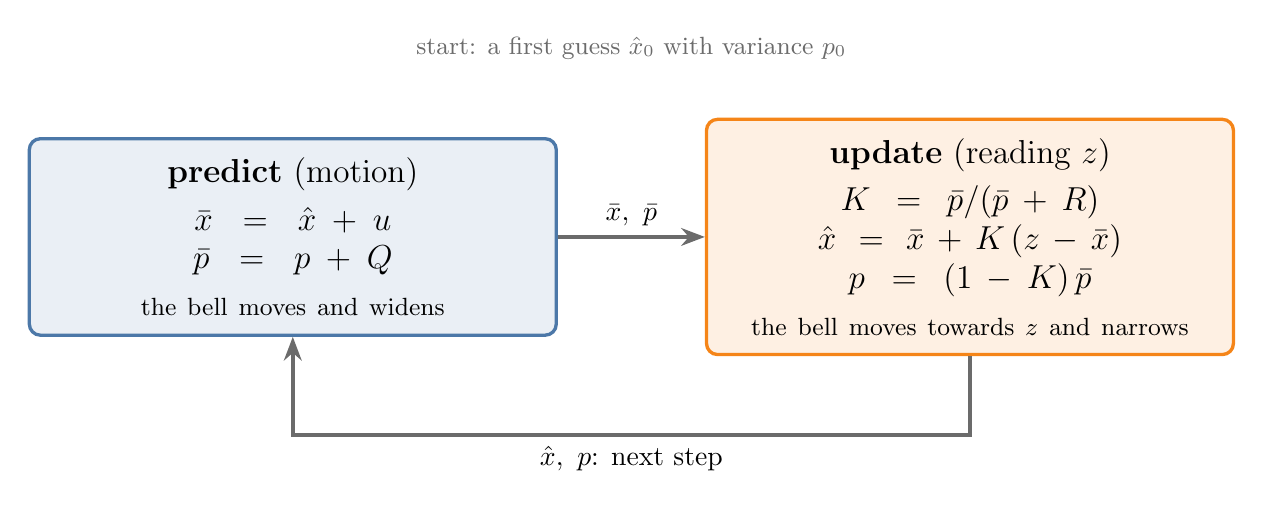
\begin{tikzpicture}[every node/.append style={font=\large}]
  \node[box=cblue, text width=6.2cm] (p) at (0,0) {\textbf{predict} (motion)\\[3pt]
     $\bar{x} = \hat{x} + u$\\ $\bar{p} = p + Q$\\[3pt] \small the bell moves and widens};
  \node[box=corange, text width=6.2cm] (u) at (8.6,0) {\textbf{update} (reading $z$)\\[3pt]
     $K = \bar{p} / (\bar{p} + R)$\\ $\hat{x} = \bar{x} + K\,(z - \bar{x})$\\ $p = (1 - K)\,\bar{p}$\\[3pt]
     \small the bell moves towards $z$ and narrows};
  \draw[arrow] (p.east) -- node[above, font=\normalsize] {$\bar{x},\ \bar{p}$} (u.west);
  \draw[arrow] (u.south) -- ++(0,-1.0) -| node[pos=0.25, below, font=\normalsize] {$\hat{x},\ p$: next step} (p.south);
  \node[note] at (4.3,2.4) {start: a first guess $\hat{x}_0$ with variance $p_0$};
\end{tikzpicture}
\end{document}
